\section{Pasta jajeczna}
\bigskip
\small
\begin{minipage}{0.45\textwidth}
    \noindent \textbf{Czas:} 15 minut \\
    \textbf{Poziom trudności:} łatwy
\end{minipage}
\begin{minipage}{0.45\textwidth}
    \noindent \textbf{Ilość sprzątania:} minimalna\\
    \textbf{Wymagany mysi sprzęt:} -
\end{minipage}
\normalsize
\vspace{0.5cm}

\begin{multicols}{2}

\subsection*{Składniki}
\begin{itemize}
    \item 3 jajka z wolnego wybiegu
    \item 1 łyżka majonezu kieleckiego, jogurtu greckiego lub mieszanki tego i tego
    \item 1 mała cebula lub garstka drobno posiekanego szczypiorku/zielonej cebulki
    \item 100 g tartego sera (np. edamski lub gouda)
    \item sól i pieprz do smaku
\end{itemize}

\columnbreak

\begin{figure}[H]
    \centering
    \fbox{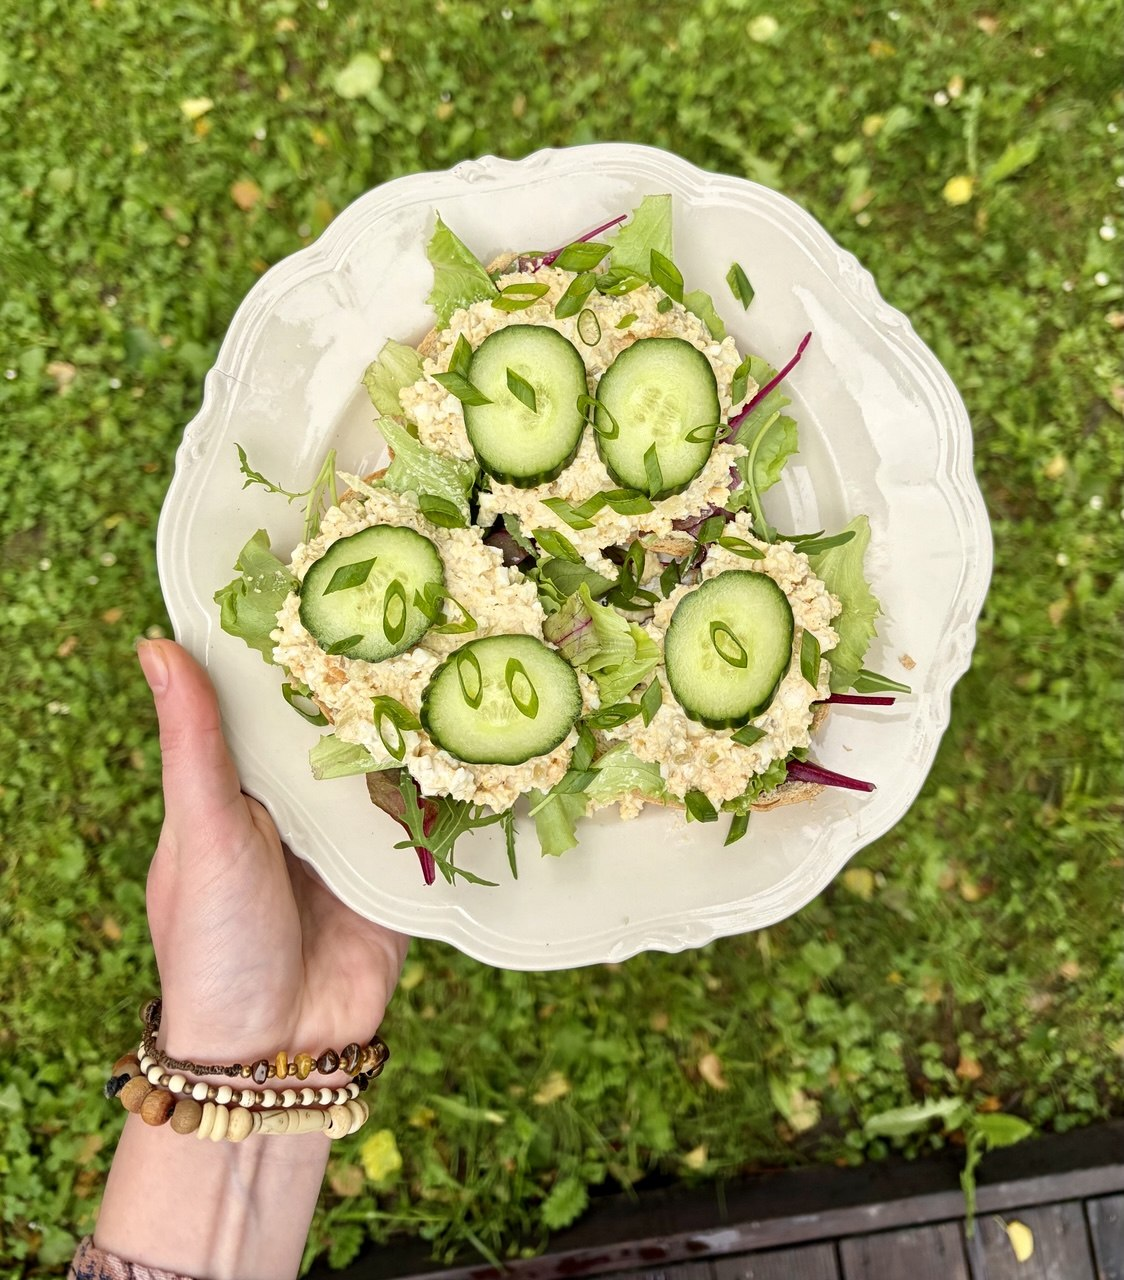
\includegraphics[width=0.35\textwidth]{images/pasta-jajeczna.jpg}}
\end{figure}
\end{multicols}

\vspace{0.5cm}

\subsection*{Instruktaż}
\begin{enumerate}
    \item Jajka ugotować na twardo. W międzyczasie posiekać cebulę na drobną kostkę i zetrzeć ser na tarce.
    \item Ostudzone jajka obrać ze skorupek, przełożyć do średniej wielkości miski i rozgniatać widelcem na drobne kawałki.
    \item Do miski z jajkami dodać pokrojoną cebulę, ser, majonez, szczyptę soli i pieprzu. Wszystko dokładnie wymieszać i w razie potrzeby doprawić do smaku większą ilością soli i/lub pieprzu bądź większą ilością majonezu do uzyskania pożądanej konsystencji.
\end{enumerate}

\vspace{0.5cm}

\small
\subsection*{Propozycja podania}
Ze świeżym chlebem, z chrupiącą sałată, z plastrami pomidora lub ogórka, z papryką

\vspace{0.3cm}

\subsection*{Dodatkowe uwagi}
Aby ostry smak surowej żółtej cebuli nie przytłaczał pozostałych składników, warto ją sparzyć - czyli posiekaną już w kawałki wrzucić do niewielkiej miseczki i zalać wrzątkiem na kilka minut. to spowoduje, że cebula w potrawach zachowa swój pyszny smak, a jednocześnie zaniknie jej nieprzyjemna ostrość.

\newpage